\documentclass[fleqn,usenatbib]{mnras}
\usepackage[utf8]{inputenc}
\usepackage{xcolor}
\usepackage{graphicx}
\usepackage{amsmath}
\title{Transient GW source number evaluation}
\author{Shu-Xu Yi}
\date{October 2018}

\begin{document}

\maketitle
The number of sources that will be detected by the telescope over a period of $T$ is calculated with the following equation:
\begin{equation}
    N=\int^T_0\int_{\rho\ge\rho^\star}\frac{dt}{1+z}dV_cd\Omega^\prime d\mathcal{M}\dot{n}(z,\mathcal{M},\theta,\varphi,i,\psi).
\end{equation}
We will explain the terms in above equation one by one:

The SNR is:
\begin{equation}
    \rho=\left(\frac{\mathcal{M}}{\mathcal{M}_0}\right)^{5/6}\frac{D_{\rm{eff},0}}{D_{\rm{eff}}}\rho_0
    \label{rho}
\end{equation}
where 
\begin{equation}
    D_{\rm{eff}}=\frac{D}{\sqrt{(\frac{1+\cos^2i}{2})^2F^2_++\cos^2iF^2_\times}}, 
\end{equation}
and $\rho_0$ is the optimized SNR with the matched-filter:
\begin{equation}
    \rho_0=2\sqrt{\int^\infty_0dt\frac{|h_0(f)|^2}{S_{\rm{n}(f)}}},
\end{equation}
where $h_0(f)$ is the GW template in Fourier domain of chirp mass $\mathcal{M}_0$ and at luminocity distance $D_{\rm{eff}}=D_0$ and optimized $i$, polarization and sky location. \footnote{Effective distance equals to luminous distance divided by the geometric terms.}

$F_{+,\times}$ is the antenna pattern functions, which are functions of source coordinates ($\theta(t)$,$\varphi(t)$) (relative to the detector, therefore is time-varing) and polarization of GW $\psi$. These terms depend on the configure of the GW detectors. 

As we can see from equation (\ref{rho}), $\rho$ is a function of $\mathcal{M}$,$D_L$,$\theta$,$\varphi$,$i$,$\psi$. In cosmological scale, $D_L$ is function of the redshift $z$. Therefore, $\rho$ is actually a function of $\mathcal{M}$,$z$,$\theta$,$\varphi$,$i$,$\psi$. And the condition that $\rho$ is no less than some threshold $\rho_\star$ constrains the region in the parameter-space of ($\mathcal{M}$,$z$,$\theta$,$\varphi$,$i$,$\psi$) to be integrated. 

$dV_c$ is the comoving volume:
\begin{equation}
    dV_c=D_H\frac{(1+z)^2D^2_A(z)}{E(z)}d\Omega dz,
\end{equation}
where 
$D_H$ is the Hubble distance, $D_A$ is the angular distance as function of $z$, $E(z)$ is function of the redshift, depends on the components of the universe. 
\begin{equation}
    d\Omega=\sin\theta d\theta d\varphi. 
\end{equation}
and 
\begin{equation}
    d\Omega^\prime=\sin idid\psi. 
\end{equation}
$\dot{n}$ is the differential co-moving event rate density in the local time. If we assume that the source is isotropic, then $\dot{n}=\dot{n}(z,\mathcal{M})$. 

Our task is 1) to find out the distribution $\textcolor{red}{\dot{n}(z,\mathcal{M})}$, and 2) to calculate the integration $\textcolor{red}{\int_{\rho\ge\rho^\star}}$. 
\section{The Distribution}
\section{The Integration}
The Integration $\int_{\rho\ge\rho^\star}$ can be calculated by defining a new function:
\begin{equation}
f(z,\mathcal{M},\theta,\varphi,i,\psi)=
    \begin{cases} 
      0 & \rho(z,\mathcal{M},\theta,\varphi,i,\psi)<\rho^\star \\
      1 & \rho(z,\mathcal{M},\theta,\varphi,i,\psi)\ge\rho^\star
    \end{cases}
\end{equation}
Then
\begin{equation}
    N=D_H\int^T_0dt\int\frac{1}{1+z}\frac{(1+z)^2D^2_A(z)}{E(z)}\dot{n}(z,\mathcal{M})f(\rho)d\Omega d\Omega^\prime dzd\mathcal{M},
\end{equation}
The above integration can be calculated with MCMC method. We draw sample points from the parameter space according to the distribution proportional to 
\begin{equation}
    \frac{(1+z)D^2_A(z)}{E(z)}\dot{n}(z,\mathcal{M}),
\end{equation}
using Markov Chain algorithm and we calculate the average of $f(\rho)$ over the sampled points. 
\section{An example calculation}
Considering the case of double neutron stars merger observing via the Einstein telescope. We assume the merger rate distribution function to be:
\begin{equation}
    \dot{n}=\dot{n}_0G(\mathcal{M},\mu,\sigma),
\end{equation}
where $G$ is function of the chirp mass, a Gaussian distribution with the mean $\mu$ and root variance $\sigma$. This distribution is assumed to be independent of the redshift $z$. The possibility distribution that the samples are draw from is:
\begin{equation}
    p(z,\mathcal{M})=\frac{(1+z)D^2_A(z)}{E(z)}\dot{n}(z,\mathcal{M})/\mathcal{N}, 
\end{equation}
where $M$ is the normalization: 
\begin{align}
    \mathcal{N}&=\int\int\frac{(1+z)D^2_A(z)}{E(z)}\dot{n}(z,\mathcal{M})dzd\mathcal{M}\\\nonumber
               &=\dot{n}_0\int\frac{(1+z)D^2_A(z)}{E(z)}dz
\end{align}
The above integration can not be done analytically, therefore we do it numerically.  We choice a high cut-off of red shift at $z=100$, and we use $\Omega_\Lambda=0.683$, $\Omega_M=1-\Omega_\Lambda$, the reduced Hubble constant $h_0=0.7$. Under theses settings, the normalization is:
\begin{equation}
    \mathcal{N}=0.93\dot{n}_0D^2_H
\end{equation}
Therefore, the number of detection is:
\begin{equation}
    N=0.93\dot{n}_0D_H^3\left<f(\rho)\right>T,
    \label{eqn:number}
\end{equation}
where the average $<...>$ is the calculated in the sample draw with the probability distribution $p(z,\mathcal{M})$. 
In order to evaluate $f(\rho)$, we want to calculate $\rho_0$, and then we scale the $\rho$ corresponding to other $\mathcal{M}$ and $D_{\rm{eff}}$ to $\rho_0$ with equation (\ref{rho})\footnote{Equation (2) cannot be used to scale $\mathcal{M}$ in a large range. It's because the masses will not also influence the normalization of the template but also the shape. Therefore $\rho_0$ is actually the function of $\mathcal{M}$ as well. Here as we're considering the double neutron star merger, the range of the chirp mass ought to be narrow. Therefore we use that method for simplification}. 

$\rho_0$ is calculated with $\mathcal{M}=1.31\,M_\odot$ (corresponds to neutron star with mass $1.5\,M_\odot$), $D_0=1$\,Mpc, with optimal sky position , inclination and polarization angle. \textcolor{red}{$\rho_0=5.1\times10^4$.} \footnote{The method of calculation: check the document ``Logic of GWtoolkit.pdf" and jupyter notebook ``SNR$\_$neutron.ipynb"} Since we are now calculating the maximum SNR we can get, we're supposing that the template are exactly matching with the source waveform. In this case we don't need a very accurate template for our purpose. As an example, we calculated $<f(\rho)>$ at $\rho^\star=10$. It gives: \textcolor{red}{$<f(\rho)>=2.7\times10^{-3}$},\footnote{Which means the ET can see 0.27\% of the whole universe of neutron stars merger events}. We use $n_0=1.3\times10^{-4}\,\text{Mpc}^3\text{yr}^{-1}$ \citep{2012ApJ...760...12A}. Therefore, put them together with equation (\ref{eqn:number}), we have \textcolor{red}{$N/T\sim2.9\times10^3/\text{yr}=7.9/\text{day}$}. 
\begin{figure}
    \centering
    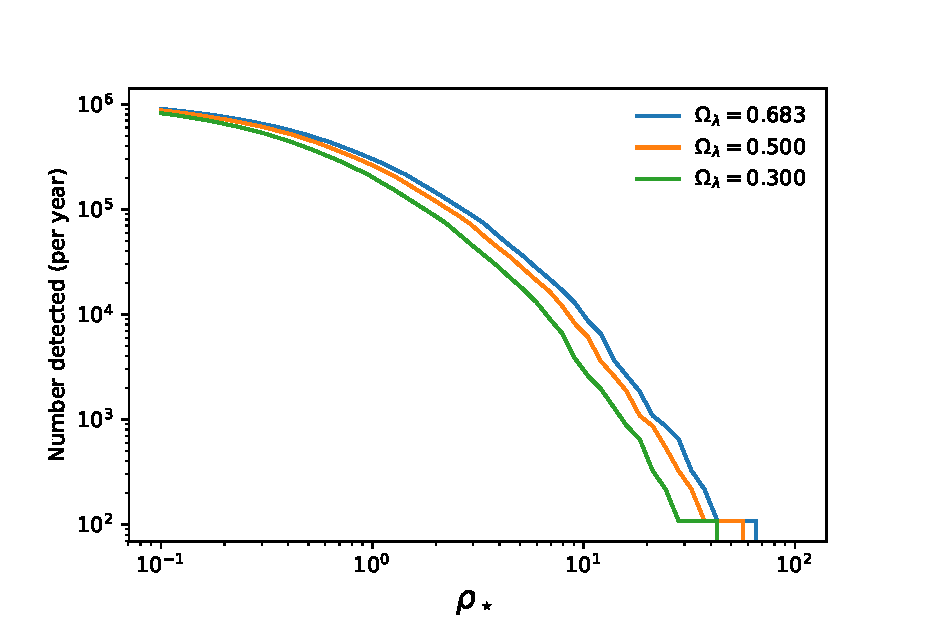
\includegraphics[width=7cm]{NvsR.eps}
    \caption{The number of detection per year as function of the criterion $\rho_\star$. Different curves correspond to different values of $\Omega_\lambda$}
    \label{fig:my_label}
\end{figure}
%We draw samples in parameter space following the distribution:
%\begin{equation}
%    p(z,\mathcal{M},\theta,\varphi,i,\psi)\propto\dot{n}(z,\mathcal{M})f(\rho),
%\end{equation}
%And we calculate the averaged value of 
%\begin{equation}
%    \frac{(1+z)D^2_A}{E}
%\end{equation}
%among the sampled points. 
\begin{thebibliography}{99}
\bibitem[Abadie et al.(2012)]{2012ApJ...760...12A} Abadie, J., Abbott, B.~P., Abbott, R., et al.\ 2012, \apj, 760, 12
\end{thebibliography}
\end{document}
